\documentclass{beamer}
\mode<presentation> { \setbeamercovered{transparent} }
\usetheme{Boadilla}

% instruct minted to use our local theorem.py
\usepackage[outputdir=build]{minted}
\usemintedstyle{tango}  % a nice, colorful theme
\setminted[lean]{bgcolor=white!83!black, fontsize=\footnotesize}
\setmintedinline[lean]{bgcolor=white!83!black, fontsize=\footnotesize}

\usepackage{template}
\usepackage{emoji}
\addbibresource{local.bib}

% \usepackage{subfiles}

\title{Formalising large corner-free sets}
\subtitle{A journey in type theory, effective topos, constructive logic and more}
\author{Gareth Ma}
\institute{University of Warwick}
\date{\today}

\linespread{1.25}

\begin{document}

\titlepage
\pagebreak

\setemojifont{Apple Color Emoji}
\setcounter{tocdepth}{1}

% part 0: intro
% formalise proof in Lean
% come up with some cool motto or something
%! TEX root = main.tex

\subsection{Imagine...}
\begin{frame}\frametitle{\insertsubsection}

You are Andrew Wiles.

You worked on a marvelous proof on a conjecture for \(6\) years, and finally publish it.

Two months later, a critical flaw was discovered, and your work is voided. \emoji{frowning-face}

If only that computers can verify Mathematical proofs...

\end{frame}



\subsection{Formalise? What?}
\begin{frame}\frametitle{\insertsubsection}

We can \textbf{formalise} proofs. Informally, it means to

\begin{definition}
  Rewrite Mathematical proofs in a machine-understandable language.
\end{definition}

The language I used is the \texttt{Lean 4} language + its Mathematics library \texttt{Mathlib 4}.

\end{frame}



\subsection{Formalise? What? \emoji{eyes}}
\begin{frame}\frametitle{\insertsubsection}

\begin{block}{Transitivity}
  Let \(P, Q, R\) be \textit{logical} statements. If \(P \implies Q\) and \(Q \implies R\), then \(P \implies R\).
\end{block}

\begin{proof}
  Suppose \(P\) holds. Then by \(P \implies Q\), we know that \(Q\) holds. And since \(Q \implies R\), we know that \(R\) holds. Hence, \(P\) implies \(R\).
\end{proof}

\begin{figure}
  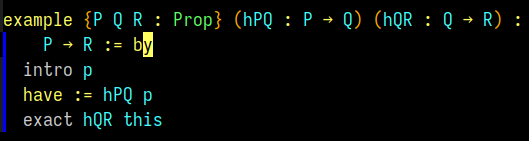
\includegraphics[scale=0.6]{images/demo.png}
\end{figure}

\end{frame}



% \subsection{Formalise? Why?}
% \begin{frame}\frametitle{\insertsubsection}
%
% \begin{enumerate}
%   \item Now: Build up mathematical library
%   \item Now/Future: Verify more complicated proofs (in real time!)
%   \item Fun!
% \end{enumerate}
%
% \end{frame}



\subsection{Formalise what? (My project)}
\begin{frame}\frametitle{\insertsubsection}

For my 3\textsuperscript{rd} year project, I formalised a extremal combinatorics result in 2021 by Ben Green.

The resulting project is original work building on top of the \texttt{Lean 4 + Mathlib 4} libraries.

To my knowledge, this is the \textbf{best} result of this type formalised in any theorem prover.

\end{frame}


\tableofcontents

% part 1: tt (section 2)
% 1.1: introduce type theory
% probably leave out all the judgement stuff
% start with set theory examples, and transfer to type theory
% give an example that's useful
% (maybe with vector spaces etc, U -> V, V -> W)
% oh also drop dependent type theory, seems not important
% in turn, also ignore the Gentzen notation stuff
% just deal with plain functions and lemmas
% definitely drop filters
% and then replace U, V, W with props and go into next part
% 1.2: curry-howard correspondence
% p -> q \and q -> r thing to talk about functions <-> (constructive) logic
% be brief here...
%! TEX root = main.tex

\section{Type Theory}

\subsection{Flaws of set theory}
\begin{frame}\frametitle{\insertsubsection}

In (naive) set theory, everything is a set. Numbers are encoded as nested sets, operations are set functions, etc.

There are many problems:

\begin{itemize}

\item \(3 \subseteq 17\) is a valid question.

\item Russell's Paradox: \(A \in A\) holds.

\end{itemize}

\end{frame}




\begin{frame}\frametitle{\insertsubsection}

Slightly absurdly, the problem fundamentally stems from that \textbf{everything is a set}.

\begin{exampleblock}{Idea}



\end{exampleblock}

\end{frame}


% part 2: math, corner-free sets (section 4-5)
% first introduce the problem
% what are corner-free sets? what is the main result?
% sketch the proof, highlighting main points
%! TEX root = main.tex

\section{Corner-free Sets}

\begin{frame}\frametitle{\insertsubsection}

\begin{block}{Corner-free sets}

  A set \(S \subseteq \Z^2\) is a corner-free set if for all \(x, y, d \in \Z\),

\[
  \{(x, y), (x, y + d), (x + d, y)\} \subseteq \S \implies d = 0
\]

\end{block}

\end{frame}


\begin{frame}\frametitle{\insertsubsection}

Apart from corner-free sets, \(3\)-AP-free sets are also commonly studied in extremal combinatorics. In my essay, I unified the approaches taken to construct the state-of-the-art lower bounds for both structures. For corner-free sets, an outline is given as follows:

\begin{enumerate}
  \item Constructing an appropriate corner-free ``two-dimensional'' additive semiring \(X = X_{r, q, d} \subseteq \Z_q^d \times \Z_q^d\) with special properties, parametrised by certain parameters \(r, q, d\);
  \item Use the naive embedding \(\zeta : \Z_q^d \to \Z\) by parsing vectors as base-\(q\) digits of integers;
  \item Prove that for \((\zeta(x), \zeta(y)), (\zeta(x'), \zeta(y)), (\zeta(x), \zeta(y')) \in \widetilde{\zeta}(X)\), \(\zeta(x') + \zeta(y) = \zeta(x) + \zeta(y') \implies x' + y = x + y'\) (using the special properties of construction);
  \item Conclude that \(\widetilde{\zeta}(X)\) is also cornerfree;
  \item Optimise parameters.
\end{enumerate}

\end{frame}


% part 3: asymptotics (section 3)
% blablabla
% dot notation seems cool (p.26), maybe demo that?
%! TEX root = main.tex

\section{Asymptotics}
\begin{frame}\frametitle{\insertsubsection}

Good luck to me. Live demo time!

\end{frame}



% part 4: verifying correctness via eval, decide and slim_check
% first introduce what decidability means (in Lean)
% simplest example is again IsSquare 37
% talk about how IsCornerFree is made decidable
% live demo time! #eval A (d := 2) (q := 4) 5 seems good
% mention how it's also useful during development: slim_check
%! TEX root = main.tex

\section{Correctness via decidability instances}
\begin{frame}\frametitle{\insertsubsection}

Good luck to me. Live demo time!

\end{frame}



% part 5: conclude
%! TEX root = main.tex

\section{Conclusion}
\begin{frame}\frametitle{\insertsubsection}

\end{frame}


\end{document}

